\section{System Overview}

\begin{outline}
  Present a high-level overview of your proposed control framework,
  likely including a block diagram (similar to Figure 1 in the
  proposal) and a description of each component.
\end{outline}

This work presents a control framework for quadruped robots that
can generate dynamic, acyclic gaits in challenging environments. The
framework is hierarchal, taking in robot state and terrain data and
outputting footstep commands to the robot controller. The first stage of
the framework is a footstep evaluation network, similar to ContactNet
from \cite{bratta_contactnet_2024}, which estimates footstep candidates
$\mathbf f_c$.
The second stage is a gait generation
network (ContactNet), which takes in footstep candidates $\mathbf f_c$,
ranks them, and finally sends the best footstep action $\mathbf f_a$ to the
robot controller.

This hierarchal framework allows for strict control over the possible
actions the robot can take. Between the two stages, the candidate
actions are filtered to ensure that the robot can only take prescribed
actions.

\begin{todo}
  update \autoref{fig:diagram-control-system}
\end{todo}

\begin{figure}[H]
  \centering
  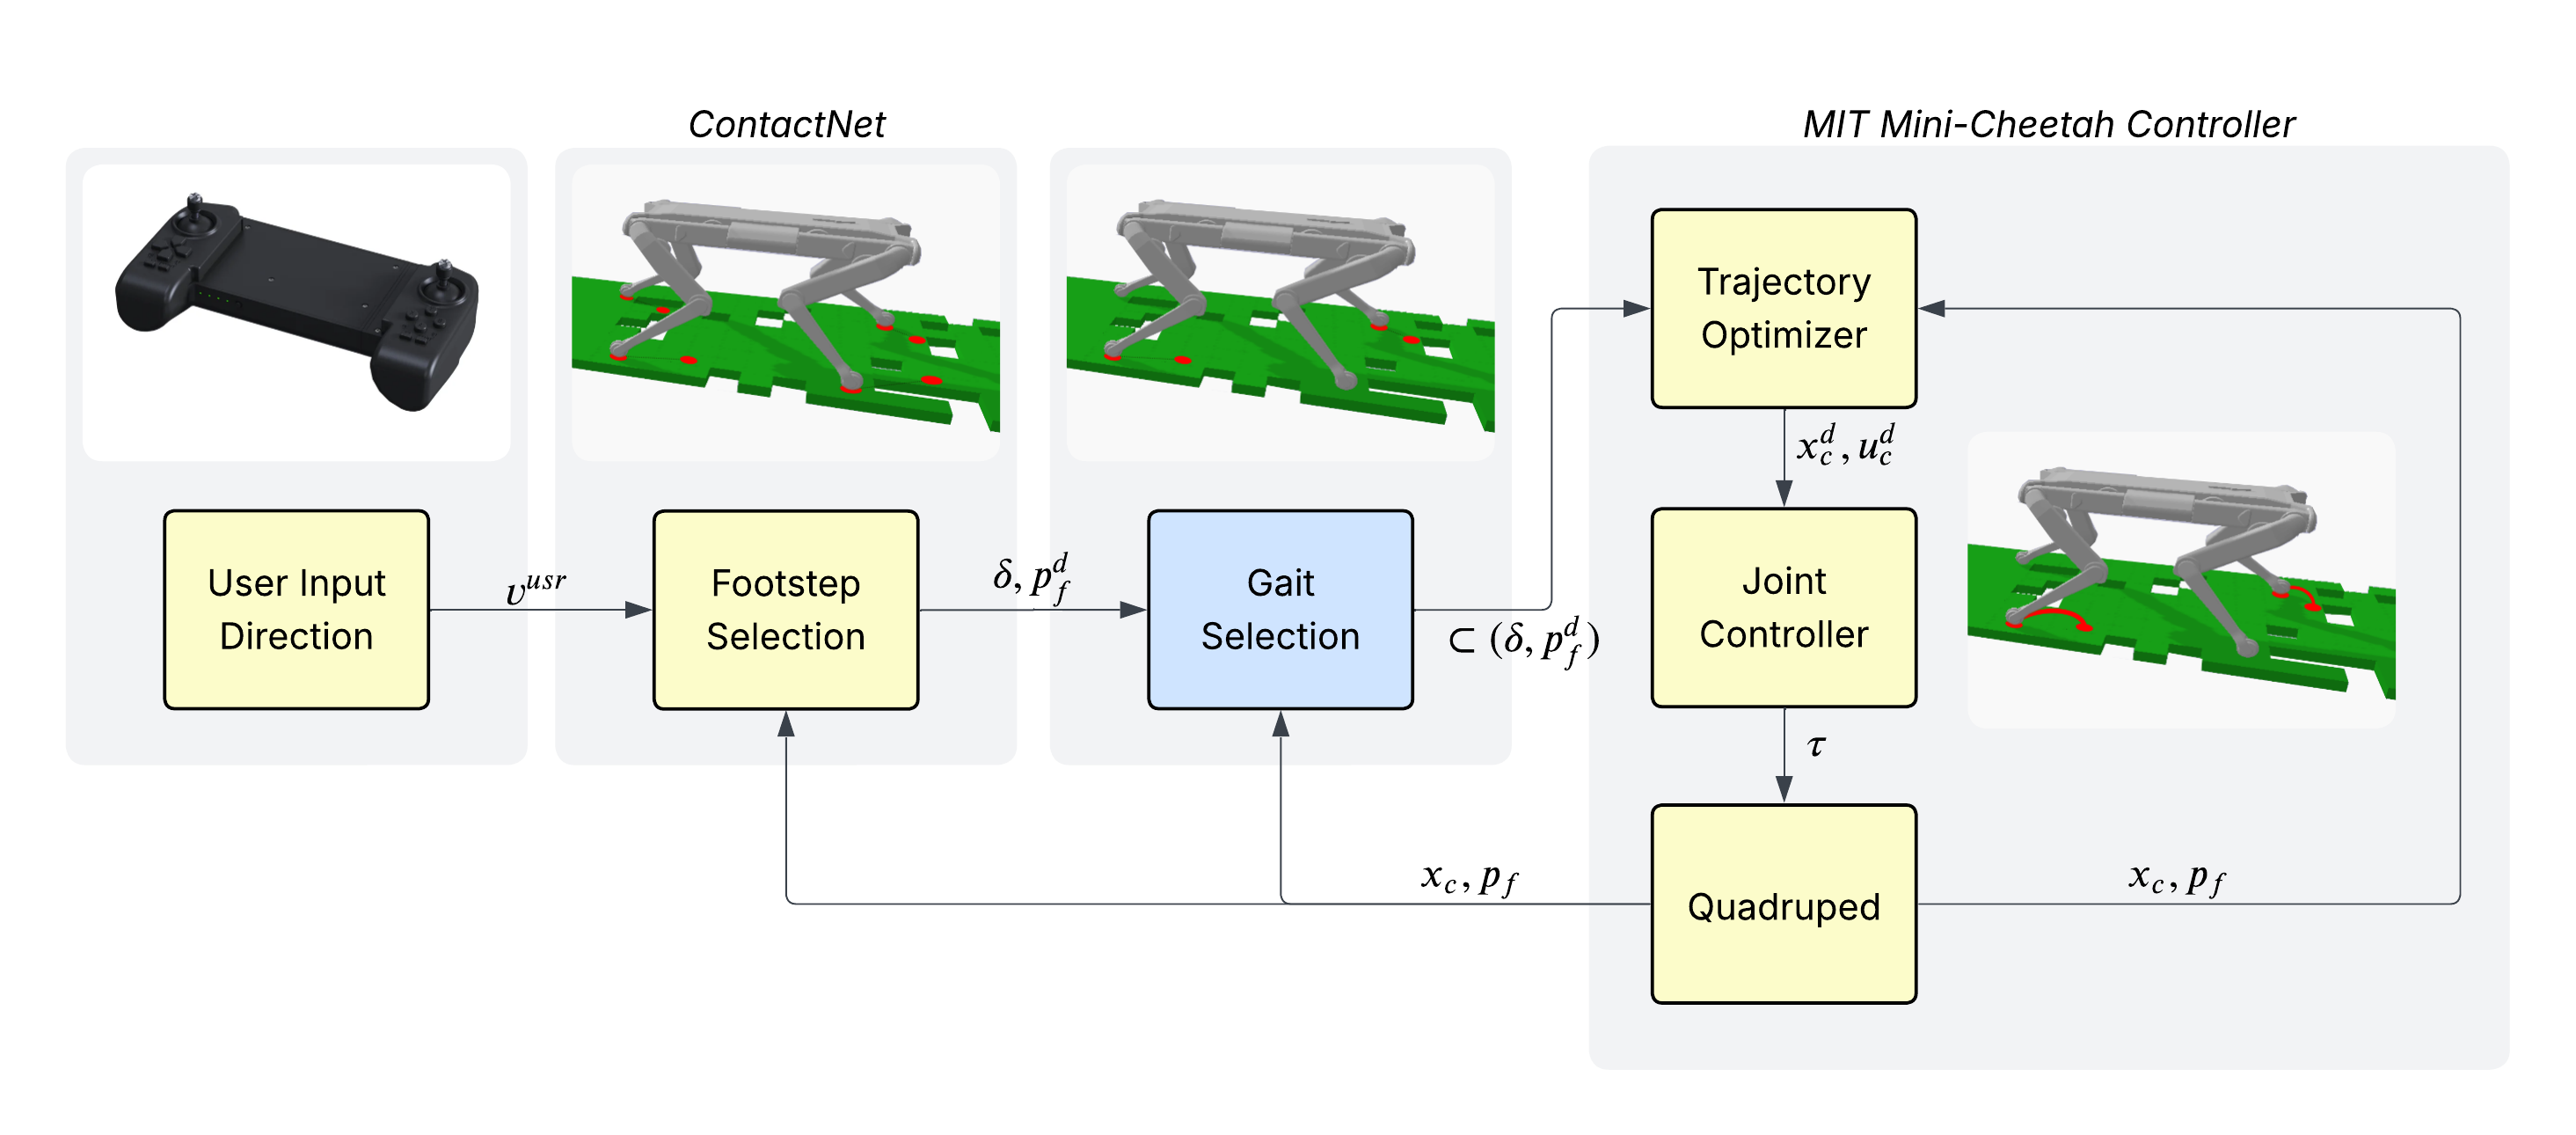
\includegraphics[width=1.0\linewidth]{images/diagrams/control-system.png}
  \caption{A block diagram of the proposed framework. The user
    defines an input direction $v^{usr}$ which the \textit{footstep
    selector} \cite{bratta_contactnet_2024} uses along with, the robot
    state $x_c$, and the current foot positions $p_f$ to generate the
    swing durations $\delta$ and touchdown points $p_f^d$ for all
    currently grounded feet. The \textit{gait selector} (novel) takes
    these desired foot movements and selects an appropriate subset
    $\subset(\delta,p_f^d)$ based on $x_c$, $p_f$, and the terrain
    data. $\subset(\delta,p_f^d)$ is then passed into the MIT
  Mini-Cheetah Controller as MPC constraints to perform lower level control.}
  \label{fig:diagram-control-system}
\end{figure}
